Finden Sie die kritischen Punkte des zweidimensionalen
Differentialgleichungssystems
\begin{equation}
\frac{d}{dx}\begin{pmatrix}y_1\\y_2\end{pmatrix}
=
\begin{pmatrix}
y_2(y_1-y_2)(1-y_2)\\
y_1(1-y_1-y_2)(1-y_1)
\end{pmatrix}
\label{602:dgl}
\end{equation}
und bestimmen sie, welche stabil und welche instabil sind.

\begin{loesung}
\begin{figure}
\centering
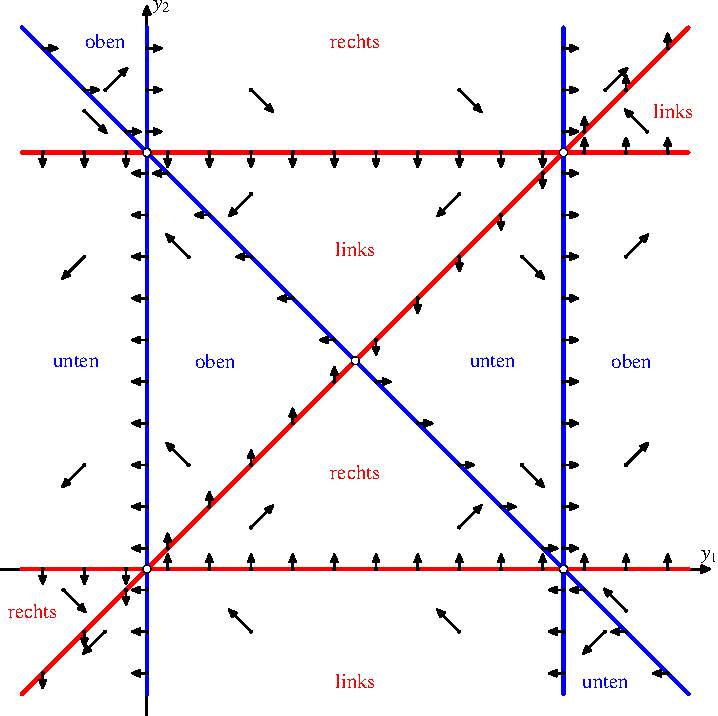
\includegraphics{../skript/uebungsaufgaben/602-1.pdf}
\caption{Nullklinen der Differentiagleichung~(\ref{602:dgl}).
\label{602:nullklinen}}
\end{figure}
Wir m"ussen die Nullklinen bestimmen.
Die $y_1$-Nullkline erf"ullt die Gleichung
\[
0=y_2(y_1-y_2)(1-y_2)
\qquad\Rightarrow\qquad
y_2=0
\quad\text{oder}\quad
y_1=y_2
\quad\text{oder}\quad
y_2=1.
\]
Die $y_2$-Nullklinen erf"ullt die Gleichung
\[
0=y_1(1-y_1-y_2)(1-y_1)
\qquad\Rightarrow\qquad
y_1=0
\quad\text{oder}\quad
y_1+y_2=1
\quad\text{oder}\quad
y_1=1.
\]
Die Abbildung~\ref{602:nullklinen} zeigt die Nullklinen dieses
Differentialgleichungssystems. 
Kritische Punkte sind Schnittpunkte verschiedenfarbiger Nullklinen.

Die Punkte $(0,1)$ und $(1,0)$ k"onnen nicht stabil sein, denn Punkte
links unterhalb von $(0,1)$ und rechts oberhalb von $(1,0)$ entfernen sich.
Der Punkt $(\frac12,\frac12)$ ist ebenfalls nicht stabil, weil sich die
Punkte $(\frac12\pm\varepsilon,\frac12)$ in der N"ahe des Punktes
$(\frac12,\frac12)$ davon entfernen.
Somit bleiben nur die Punkte $(0,0)$ und $(1,1)$ konnen nicht
stabil sein, weil sich Punkte rechts oberhalb von $(1,1)$ 
und links unterhalb von $(0,0)$ ebenfalls entfernen.
Alle f"unf kritischen Punkte sind daher instabil.
\end{loesung}

